\documentclass[conference]{IEEEtran}
\IEEEoverridecommandlockouts
% The preceding line is only needed to identify funding in the first footnote. If that is unneeded, please comment it out.
\usepackage{cite}
\usepackage{amsmath,amssymb,amsfonts}
\usepackage{algorithmic}
\usepackage{graphicx}
\usepackage{textcomp}
\usepackage{xcolor}
\usepackage[colorlinks=true,linkcolor=blue,urlcolor=cyan]{hyperref}

\def\BibTeX{{\rm B\kern-.05em{\sc i\kern-.025em b}\kern-.08em
    T\kern-.1667em\lower.7ex\hbox{E}\kern-.125emX}}
\begin{document}

\title{A Hybrid Approach to Scientific Software Package Management on a High Performance Computing Cluster\\
}

\author{\IEEEauthorblockN{1\textsuperscript{st} Qiyang Hu}
\IEEEauthorblockA{\textit{Institute for Digital Research and Education} \\
\textit{University Of California, Los Angeles}\\
Los Angeles, California, USA \\
huqy@idre.ucla.edu}
\and
\IEEEauthorblockN{2\textsuperscript{nd} Shao-Ching Huang}
\IEEEauthorblockA{\textit{Institute for Digital Research and Education} \\
\textit{University Of California, Los Angeles}\\
Los Angeles, California, USA \\
schuang@idre.ucla.edu}
}

\maketitle

\begin{abstract}
This paper describes a new approach for managing the computational packages in an HPC cluster environment.
In Section~\ref{sec_intro}, we first reviewed the system administration challenges to manage HPC applications in using traditional naive building way and the software management approach. Our work's goal and the paper's contribution were also clarified.
We then discuss on a way to have an interface to hybridize both Spack and manual software installation ways to provide a better presentation to users as a proof of concept in Section~\ref{sec_modulefiles}. A typical workflow is proposed in Section~\ref{sec_workflow}.  
A brief conclusion is summarized in Section~\ref{sec_summary}.

\end{abstract}

\begin{IEEEkeywords}
Spack, software management, modules, HPC 
\end{IEEEkeywords}

\section{Introduction}\label{sec_intro}

%%{\color{gray}(1) General challenge}
Keeping scientific computing software packages up-to-date and easy to use for users is of ultimate importance of the success of a computing cluster's operation.
In practice, this posses a challenge on a operational team.
Especially when the number of scientific packages in an HPC environment is large, keeping every software deployment up to date for new releases and providing the persistent supports to the diverse needs from users become a tedious and time-consuming process. 
The combinatorial nameing and versioning complexities easily get exploded among hundreds of package sets, module files and corresponding documents maintained by multiple system admins. 
%%{\color{gray}(2) framework solution's advantages}
The common solution for the above challenges is to use an software management framework (e.g. EasyBuild and Spack) to simplify or automate a significant amount of mundane work. 
With the systemmatic way of configuring, building and deploying application packages, the framework approach shows to be promising to largely improve HPC cluster's operational efficiency. 

%%{\color{gray}(3) framework solution's limitations}
However, as all the software management frameworks are still in a rapid development stage, a few limitations from the framework approach make it hard to serve as a solely suite along to manage software packages in practical sense.
One of the issues for cluster system admins is that the restrictions from the frameworks are too rigid, even for the most flexible framework solution (Spack) and it make it not easy to plug into the existing software stack with the legacy system configurations. 
Module naming schemes that differed from naive installation naming conventions required complex configuration to adapt to existing manual installation scheme. It is always difficult to manage software and dependencies built outside of the tools. 
Another issue is that the systematic handling on various library dependencies results in many duplicate builds of the same software which introduces unnecesary confusions in the end user level experience. 
The complexity of configurations in those frameworks is another stopping force where some functionalities are not mature enough for dealing with all the corner cases. It would be a challenge for finding a way to both take advantage of the powerful capability of framework approach and keep compatability with the existing naive approach.  

%%{\color{gray}(4) our approach and values/contributions of our work}
In this paper we propose a practical approach for HPC cluster admins to manage software packages by hybridizing the framework approach and the naive installation approach. 
Our central idea is to construct a higher layer above the software framework, where a mechanism is introduced to manage applications built from the framework and from manual installation to make the flexible customization possible to accomodate the existing software infrastructures in HPC cluster environment.
Specifically, we select Spack as the candidate of package management framework tool and the practice of traditional naive package building environment is taken in UCLA high performance cluster Hoffman2.  
We try to keep the spack and manually-installed system decoupling as possible as it could, so that it will hopefully give the enough time for frameworks to develop further while not halting the adoption right now. 
Our major work is the creative ways to manipulate and re-organize the module files and propose a practical workflow to manage the building and maintaining process in a maximum scriptable/automatic way and provide a neat presentation interface to end users.


\section{Managing Module Files} \label{sec_modulefiles}

\subsection{Pros, cons and solutions}

From our practice on working with Spack and our experience on managing module files for manually installed packages, we noticed that there are pros and cons for both methods. In Spack, module files are automatically generated during the installation and it systematically collects all dependent libraries and provide the corresponding modules, which is a big advantage. The structure and format for module files are controlled by Spack's yaml script. However the customization configuration is very limited and not flexible enough to meet the needs, especially:

\begin{itemize}
    \item Flat structure of module files are only for \texttt{tcl} format, while Hierarchical structure are only for \texttt{lua} format.
    \item Due to the systematic installation, the minor tweaks of flags and options for the same packages will be considered as different versions. However the naming scheme from Spack yaml script is impossible to cover all the cases. Thus the Spack installation process produces tons of duplication of installed packages/libs. The canonical solution from Spack is to assign a unique hash code for every version of all packages. The end result is that the module file presentation from Spack is confusing to general users with a lot of seemingly redundant duplication packages with lacking of direct and explicit ways to expose the information to users.
    \item Hierarchical structure generated from Spack is fixed, there is currently no way to customize.
\end{itemize}

As to module files for manual package installation, the flexibility is the biggest advantage. At least 1/3 of packages have to be dealt with the manual way. However our current hierarchical module structure is just verbally defined. Because every module file needs to be written by hand, it lacks a strict way to reinforce the hierarchy. Also because we are currently using TCL-based module files, the hierarchical structure has to be implemented by hacking tricks inside the module files. At the same time, some safety features have to be implemented manually, for example, for restricting one version of a module can be activated at one time, or only one compiler and/or mpi can be loaded at one time.

Our solution to this situation is to provide an interface to hybridize the both system. In particular:

\begin{enumerate}
    \item We need to design a clearly defined hierarchical structure so that the modulefiles from Spack can have a unique mapping and the manually generated modulefiles can also comply the definition.
    \item We need to implement a script to process the Spack's auto-generated modulefiles so that it will do:
        \begin{itemize}
            \item Match \& copy-in Spack modulefiles to the structure
            \item Filter out the confusing duplication
            \item Filter out the packages the system admins don't want to support
            \item Redefine the version default
        \end{itemize}
    \item We need to enforce the safety features systematically. That will be easily done by replacing TCL module files with Lmod, as Lmod module system is indisputably the main choice for large scale HPC systems and a drop-in replacement for TCL/C ones \cite{mclay:11}.
\end{enumerate}

\subsection{Defining modulefile structures in user level} \label{subsec_redefine_h2_modulefiles}

As shown in Fig. \ref{fig:spack_flat} of an example that we installed on Hoffman2, the flat module file structure generated by Spack has a straight-forward naming scheme under the root place with simple listing of package names. Different installations of each package are stored in the corresponding directory as TCL/C module files with a name concatenating the application version, compiler name, compiler version, and the mpi name and version. Plus, the TCL/C module files appends the unique hash code in order to distinguish the duplication names from minor difference of installations with the same version and same compiler/mpi info.

\begin{figure}[htbp]
  \centerline{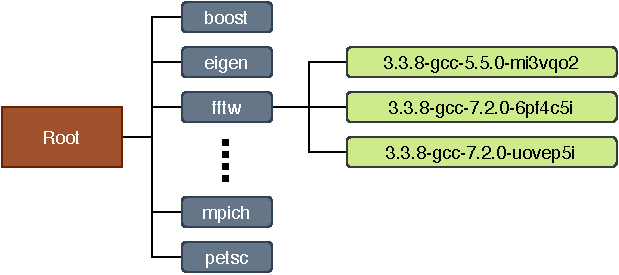
\includegraphics[width=\linewidth]{figures/spack_flat}}
  \caption{Flat structure of module files generated by Spack}
  \label{fig:spack_flat}
\end{figure}

At the same time, the hierarchical module files generated by Spack follows the typical Core/Compiler/MPI structures. Fig.~\ref{fig:spack_hier} shows an example of our modules.yaml configuration on Hoffman2. It can be noticed that the software installations are organized in a convoluted way, which means the applications under ``Core'' are the simplest with only dependency on system libraries, the ones under ``Compiler''s are dependent on the Spack-installed compilers only, the ones under ``MPI'' are dependent on both compilers and mpis. In Fig.~\ref{fig:spack_hier} we introduced customized ``openblas'' category to test the customization capabilities of Spack's modules.yaml. It can be understood as the in-between level of Compiler and MPI, which obviously adds more complexity in the MPI level directory. Every package installed is listed as a folder as its name under the corresponding directory levels. The module files for different versions are \texttt{lua} files with \texttt{.lua} extension and have a simpler name with its own version plus the unique hash code if necessary.


\begin{figure}[htbp]
  \centerline{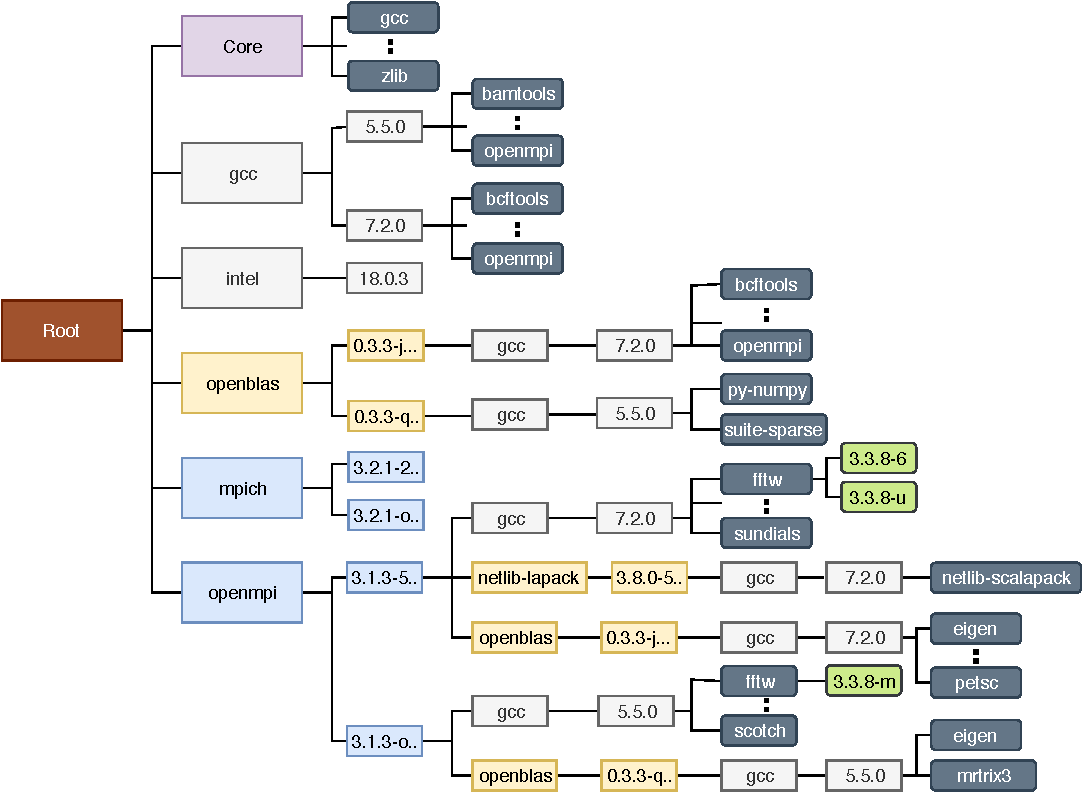
\includegraphics[width=\linewidth]{figures/spack_hier}}
  \caption{Hierarchical structure of module files generated by Spack}
  \label{fig:spack_hier}
\end{figure}


In order to get a better practical understanding on managing the module files on large scale HPC clusters, we closely inspected the module files on TACC. As shown in Fig. \ref{fig:tacc_hier}, TACC follows the Core/Compiler/MPI hierarchical structure but the MPI level is embedded inside the Compiler level. Since they still use \texttt{TCL/C} module system, they keep the traditional \texttt{modulefiles} sub-directory to contain the modulefiles for installed packages. It should be noted that they also have some special categories (e.g. \texttt{python2\_7}, \texttt{python3\_7}) as the nested levels inside the Compilers and MPIs.

\begin{figure}[htbp]
  \centerline{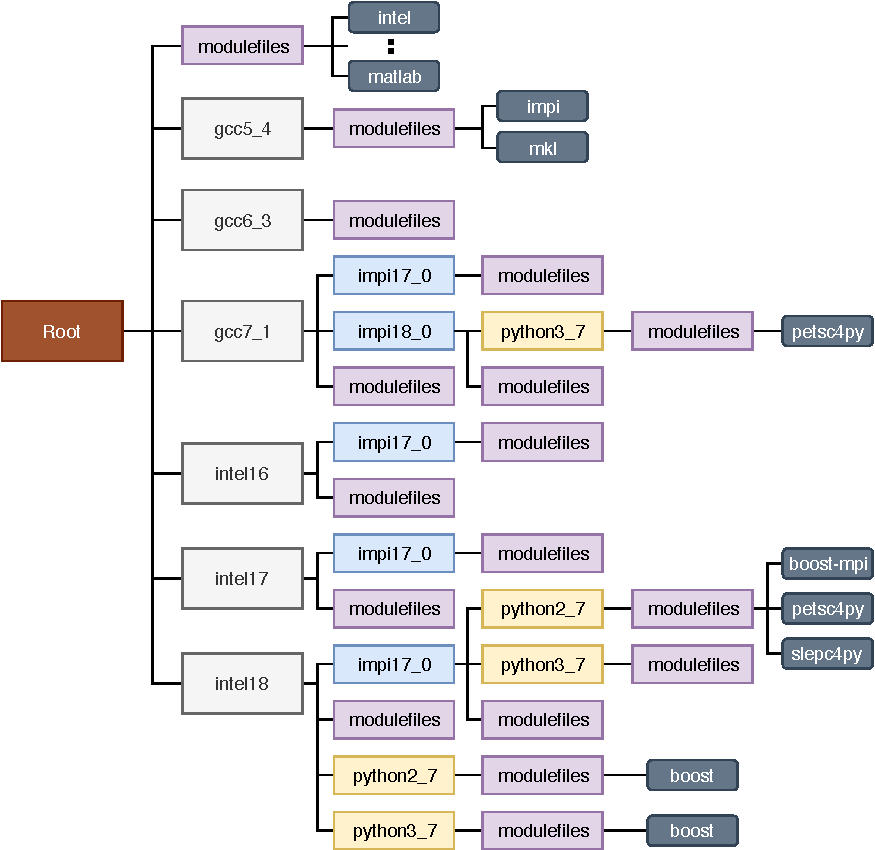
\includegraphics[width=\linewidth]{figures/tacc_hier}}
  \caption{Hierarchical structure of module files in TACC}
  \label{fig:tacc_hier}
\end{figure}

Based on the above information, we propose the module files on Hoffman2 to be organized in a simple structure as shown in Fig. \ref{fig:h2_new_hier}, where the MPI level is nested in the compiler level as TACC did. The versions of compilers and MPIs are following the convention in Spack. We will use \texttt{lua} format which means the module files will have \texttt{.lua} extension. \texttt{modulefiles} sub-directory is preserved for denoting to store the installed packages' module files from the upper directories from the corresponding compilers, or MPIs or both. The additional categories will be optional to be nested in Compiler level or Compiler+MPI levels if necessary. It can be noted that as the anaconda installation becomes a trending approach for the python packages, there will be separate from the module file system as a pre-built stack shown in Fig. \ref{fig:sw_inst_structure}.

\begin{figure}[htbp]
  \centerline{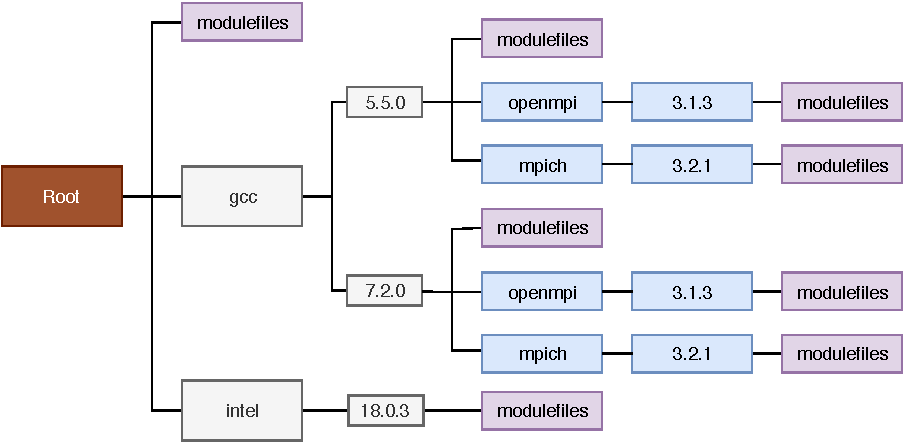
\includegraphics[width=\linewidth]{figures/h2_new_hier}}
  \caption{Newly defined hierarchical structure of module files in Hoffman2}
  \label{fig:h2_new_hier}
\end{figure}


\subsection{Python scripts for modulefile processing}\label{subsec_modulefile_processing}

The module file process means we would like to develop a script to import the module file information automatically generated from Spack, filter out the not-to-be-supported packages, make desired modifications on the to-be-supported module files and export to the destination folder which will be the default module path for general users.

Before processing the modulefiles, we propose to a JSON-format list to contain the information about the packages that the system admins plan to support. An example of a JSON file will be like below, where only 3 packages will be supported and the versions are listed by concatenating the compiler's information:

\begin{verbatim}
{   "bowtie": {
        "name_in_spack": "bowtie",
        "version": [
            "1.2-gcc-7.2.0",
            "1.2-gcc-5.5.0"
        ],
        "default": "1.2"
    },
    "bowtie2": {
        "name_in_spack": "bowtie2",
        "version": [
            "2.3.4.1-gcc-7.2.0",
            "2.3.4.1-gcc-5.5.0"
        ],
        "default": "2.3.4.1"
    },
    "gcc": {
        "name_in_spack": "gcc",
        "version": [
            "5.5.0-gcc-4.8.5",
            "7.2.0-gcc-4.8.5"
        ],
        "default": "7.2.0"
    }
}
\end{verbatim}

%%{\color{red}Add explanation of the fields (keys and values) in the JSON file and briefly why.}

As shown in the example the json file defines an array of objects. Each of the objects contains a main name-value pair, where the main name is the application name given from system admins, e.g. \verb|bowtie|, \verb|bowtie2| and \verb|gcc|. The value of the main name contains another set of name-value pair defines the information of: 

\begin{itemize}
    \item the application name used in Spack \verb|name_in_spack|. It can be blank if there is no cooresponding one in Spack.
    \item the application version that will be supported \verb|version|. The version keeps the information of compilers. In the future, it can contain the further information like MPI or Scalapack as well.
    \item the default version that will be shown or selected by the \verb|Lmod| system. It can be noted that the version here will not need the additional compiler or MPI information, because of the enforced step-down step from hierarchical structure. 
\end{itemize}

Our approach is to take advantage of Spack's capability of generating both flat and hierarchical module files by enabling them in modules.yaml configuration file. As shown in Fig. \ref{fig:modulefilter_flowchart}, we first iterate over Spack's hierarchical module structures to obtain the hierarchical information about the installed packages and the hash codes generated from Spack. All collected information will be saved in a Sqlite database file. Then we iterate over Spack's flat-structured module files to find the ones in the database with the same hash code. By cross-checking the customized JSON file to decide the display option for the packages we can make the corresponding modifications for the module files and copy it to the destination directory. The modifications specifically include:

\begin{itemize}
    \item Using \texttt{tcl2lua.tcl} script to convert the \texttt{TCL/C} module file to \texttt{lua} format.
    \item Pre-pending \texttt{MODULEPATH} to enable the dynamically showing of available module files under the corresponding Compiler/MPI directories if necessary.
    \item Adding \texttt{family} to guarantee users can only load one compiler or MPI stack at a time, if necessary.
    \item Specifying the default version for the packages by generating \texttt{.version} file in the destination package modulefile folder.
\end{itemize}

\begin{figure}[htbp]
  \centerline{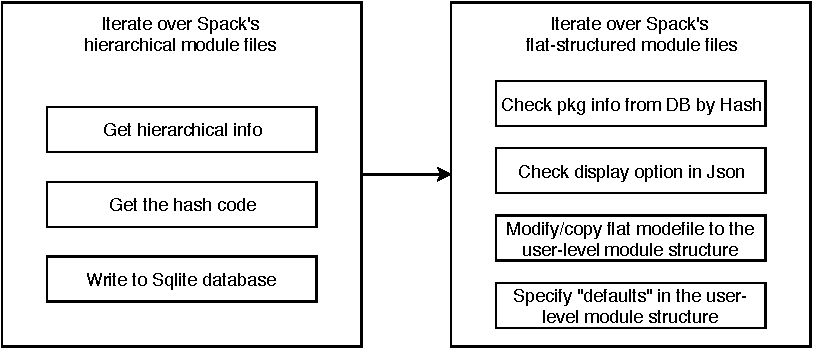
\includegraphics[width=\linewidth]{figures/modulefilter_flowchart}}
  \caption{Flowchart for the python script to generate the newly defined module file structures for user-level presentations}
  \label{fig:modulefilter_flowchart}
\end{figure}

In the SQLite database file (\verb|apps.db|), there is currently only one table (\verb|apps|) in the database. The schema of the table can be reviewed by \verb|.schema apps| inside the SQLite shell. The detailed column information is listed below:

\begin{itemize}
    \item \verb|id|: integer, primary key with autoincrement.
    \item \verb|appname|: text, the name of the application. Note: it will be the exact app's name in Spack if installed via Spack.
    \item \verb|appver|: text, the version of the application. Note: it will be the exact app's version string in Spack if installed via Spack.
    \item \verb|apphash|: text, the hash code of the installed application. Note: it will only has non-null values for packages installed via Spack. It will have NULL value for manually installed ones. Thus it can serve as the flag to know if the application installation is from Spack or manual installation.
    \item \verb|compname|: text, the name of the compiler to compile the app. Note: it will be the exact compiler's name in Spack if installed via Spack.
    \item \verb|compver|: text, the version of the compiler to compile the app. Note: it will be the exact compiler's version string in Spack if installed via Spack.
    \item \verb|mpiname|: text, the name of the MPI to compile the app. Note: it will be the exact MPI's name in Spack if installed via Spack.
    \item \verb|mpiver|: text, the version of the MPI to compile the app. Note: it will be the exact compiler's version string in Spack if installed via Spack.
    \item \verb|mpihash|: text, the hash code of the installed MPI package to compile the application. Note: it will only has non-null values for packages installed via Spack. It will have NULL value for manually installed ones. 
    \item \verb|hierpath|: text, the module file path in the hierarchical module structure. For the Spack-installed package, it will be in the Spack-defined hierarchical modulefile folder. For the manually-installed package, it will keep blank. 
    \item \verb|flatpath|: text, the module file path in the flat module structure. For the Spack-installed package, it will be in the Spack-defined hierarchical modulefile folder. For the manually-installed package, it will the customized pathes for the manually-formed module file. It should be noted that the module file from manual installation does not have to be the one for flat structure. It can be from the hierarchical one.
    \item \verb|custpath|: text, the destination path for the module file to be presented to users. It can leave blank.
    \item \verb|present|: integer, the flag to show if the module file to be presented to users. It can leave blank for module filter script to update the value according to JSON file.

\end{itemize}


We also discussed about managing the installed (built or pre-built) libraries under the specific language (R or Python) environments in the modulefile processing script. A possible way is to generate the list of installed packages/libraries for the versions of R or Anaconda Python as separate text files and provide the information about the directories in the \texttt{module show} commands. This function is not yet implemented but very doable in the picture.


\section{Hybridization of Spack- and Manually-install Packages (TODO)} \label{sec_workflow}

%%{\color{red}
%%The followings will be addressed in this section (or merge/split the discussion into other sections):
%%
%%\begin{itemize}
%%\item The workflow (or flow chart) of installing a package, from the installation request to displaying the module. The procedure of registering the package in the database also needs to be described.
%%\item How to query whether a package is covered by Spack or not, given the package's name and optional a version, in order to determine it's installation approach. This is especially important for new packages.
%%\item Describe the database schema (to the extent that the reader can understand its logical structure without looking at the DB itself in the repository), similar to the description of the JSON file.
%%\item The procedure (and script) to generate output (e.g. table) about supported packages for Hoffman2 documentation.
%%\end{itemize}
%%
%%}

The practical process to hybridize the Spack-installed and manually-installed packages can be built based on the structures that were proposed in the above section. Specifically we can use the JSON file and SQLite file defined in Section \ref{subsec_modulefile_processing} to coordinate both ways of installation. Figure \ref{fig:spack_h2_hybrid_flow} below shows one possibility of workflow of installing a package, from the installation request to displaying the module.

\begin{figure}[htbp]
  \centerline{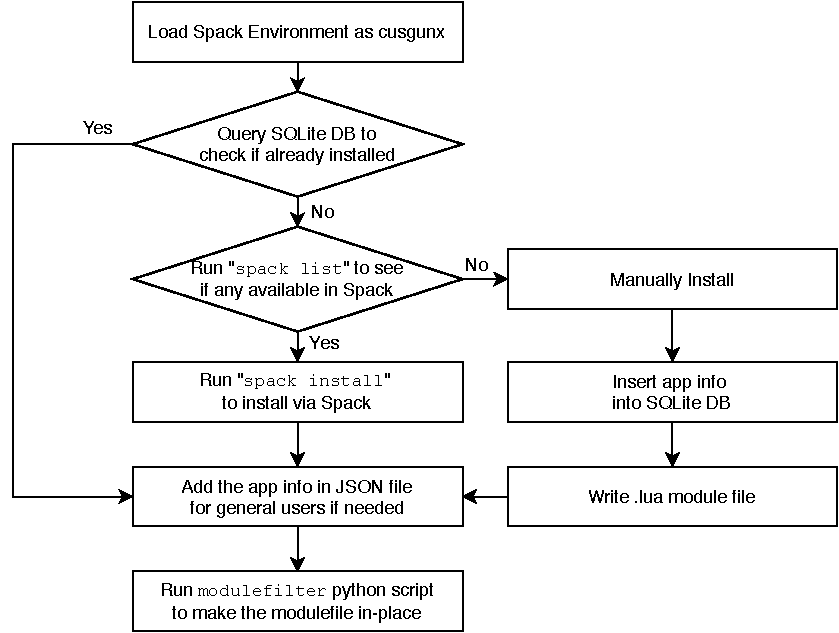
\includegraphics[width=\linewidth]{figures/spack_h2_hybrid_flow}}
  \caption{The workflow to hybridize the Spack-installed and manually-installed packages}
  \label{fig:spack_h2_hybrid_flow}
\end{figure}

The workflow shows a basic process to check and install a newly requested application into the hybrid system. A couple of notes are listed below for further explantation:

\begin{itemize}
    \item All the installation processes are assumed to be taken as \verb|cusgunx| user.
    \item With the schema information explained in Section \ref{subsec_modulefile_processing}, it would be easy to use the standard SQL \verb|select| query to check if the newly requested package with the specific requested version has been installed on Hoffman2 or not.
    \item If installation is needed, the command \verb|spack list $APPNAME| can be used to check if there is any available package whose name contains \verb|$APPNAME| Spack can install. The detailed document for \verb|spack list| command can be checked in the \href{https://spack.readthedocs.io/en/latest/command_index.html#spack-list}{link}.
    \item If Spack provides the available package to install, the command \verb|spack install $APPNAME| can be used to install it. This will be the most tricky part that needs the experience and knowledge about some specific Spack syntax. The detailed document for \verb|spack install| command can be found in the \href{https://spack.readthedocs.io/en/latest/basic_usage.html#cmd-spack-install}{link}. We already documented 180+ package installation commands for the existing software packages on Hoffman2 shown in the \href{https://ucla-my.sharepoint.com/:x:/g/personal/huqy_ad_ucla_edu/ESfMOTn1oidAlnMlAVYbCd8BOlgseFtgmbwszJPsum7AgQ?e=sGbSoJ}{spreadsheet} in Section \ref{subsec_proposed_cat_pkgs}. This will serve as a good reference. 
    \item For packages needed the manual installation, a SQL \verb|insert| command will be needed to populate the information into the database. It should be noted that the field \verb|apphash| has to leave blank as the flag to denote the installation is not from Spack.
    \item The \verb|lmod| modulefile from manually installed package will needed to be written manually as well. It can be the \verb|TCL/C|-based script or \verb|lua|-based one, since the modulefilter script will do the conversion. The directory for drafting the module file can be arbitrary but has to be consistent with the value of the \verb|flatpath| in the database record inserted above.
    \item The JSON file has to be updated according the schema described in Section \ref{subsec_modulefile_processing}. 
\end{itemize}


\section{Summary} \label{sec_summary}

In this report we documented our effort for investigating Hoffman2 Software Management during the past year. Specifically we proposed a plan for Hoffman2 software installation structure and summarize the related installation work. We also discussed a way to have an interface to hybridize both Spack and manual software installation ways to provide a better presentation to users as a proof of concept.

\begin{thebibliography}{00}
\bibitem{gamblin:15} Todd Gamblin, Matthew LeGendre, Michael R. Collette, Gregory L. Lee, Adam Moody, Bronis R. de Supinski, and Scott Futral. ``The spack package manager: bringing order to hpc software chaos,'' SC ’15 Proceedings of the International Conference for High Performance Computing, Networking, Storage and Analysis, 2015.
\bibitem{mclay:11} R. McLay, K. W. Schulz, W. L. Barth, and T. Minyard. ``Best practices for the deployment and management of production hpc clusters,'' In SC ’11 In State of the Practice Reports, page 9:1–9:11, 2011.
\end{thebibliography}

\end{document}







\section{Ease of Use}

\subsection{Maintaining the Integrity of the Specifications}

The IEEEtran class file is used to format your paper and style the text. All margins, 
column widths, line spaces, and text fonts are prescribed; please do not 
alter them. You may note peculiarities. For example, the head margin
measures proportionately more than is customary. This measurement 
and others are deliberate, using specifications that anticipate your paper 
as one part of the entire proceedings, and not as an independent document. 
Please do not revise any of the current designations.

\section{Prepare Your Paper Before Styling}
Before you begin to format your paper, first write and save the content as a 
separate text file. Complete all content and organizational editing before 
formatting. Please note sections \ref{AA}--\ref{SCM} below for more information on 
proofreading, spelling and grammar.

Keep your text and graphic files separate until after the text has been 
formatted and styled. Do not number text heads---{\LaTeX} will do that 
for you.

\subsection{Abbreviations and Acronyms}\label{AA}
Define abbreviations and acronyms the first time they are used in the text, 
even after they have been defined in the abstract. Abbreviations such as 
IEEE, SI, MKS, CGS, ac, dc, and rms do not have to be defined. Do not use 
abbreviations in the title or heads unless they are unavoidable.

\subsection{Units}
\begin{itemize}
\item Use either SI (MKS) or CGS as primary units. (SI units are encouraged.) English units may be used as secondary units (in parentheses). An exception would be the use of English units as identifiers in trade, such as ``3.5-inch disk drive''.
\item Avoid combining SI and CGS units, such as current in amperes and magnetic field in oersteds. This often leads to confusion because equations do not balance dimensionally. If you must use mixed units, clearly state the units for each quantity that you use in an equation.
\item Do not mix complete spellings and abbreviations of units: ``Wb/m\textsuperscript{2}'' or ``webers per square meter'', not ``webers/m\textsuperscript{2}''. Spell out units when they appear in text: ``. . . a few henries'', not ``. . . a few H''.
\item Use a zero before decimal points: ``0.25'', not ``.25''. Use ``cm\textsuperscript{3}'', not ``cc''.)
\end{itemize}

\subsection{Equations}
Number equations consecutively. To make your 
equations more compact, you may use the solidus (~/~), the exp function, or 
appropriate exponents. Italicize Roman symbols for quantities and variables, 
but not Greek symbols. Use a long dash rather than a hyphen for a minus 
sign. Punctuate equations with commas or periods when they are part of a 
sentence, as in:
\begin{equation}
a+b=\gamma\label{eq}
\end{equation}

Be sure that the 
symbols in your equation have been defined before or immediately following 
the equation. Use ``\eqref{eq}'', not ``Eq.~\eqref{eq}'' or ``equation \eqref{eq}'', except at 
the beginning of a sentence: ``Equation \eqref{eq} is . . .''

\subsection{\LaTeX-Specific Advice}

Please use ``soft'' (e.g., \verb|\eqref{Eq}|) cross references instead
of ``hard'' references (e.g., \verb|(1)|). That will make it possible
to combine sections, add equations, or change the order of figures or
citations without having to go through the file line by line.

Please don't use the \verb|{eqnarray}| equation environment. Use
\verb|{align}| or \verb|{IEEEeqnarray}| instead. The \verb|{eqnarray}|
environment leaves unsightly spaces around relation symbols.

Please note that the \verb|{subequations}| environment in {\LaTeX}
will increment the main equation counter even when there are no
equation numbers displayed. If you forget that, you might write an
article in which the equation numbers skip from (17) to (20), causing
the copy editors to wonder if you've discovered a new method of
counting.

{\BibTeX} does not work by magic. It doesn't get the bibliographic
data from thin air but from .bib files. If you use {\BibTeX} to produce a
bibliography you must send the .bib files. 

{\LaTeX} can't read your mind. If you assign the same label to a
subsubsection and a table, you might find that Table I has been cross
referenced as Table IV-B3. 

{\LaTeX} does not have precognitive abilities. If you put a
\verb|\label| command before the command that updates the counter it's
supposed to be using, the label will pick up the last counter to be
cross referenced instead. In particular, a \verb|\label| command
should not go before the caption of a figure or a table.

Do not use \verb|\nonumber| inside the \verb|{array}| environment. It
will not stop equation numbers inside \verb|{array}| (there won't be
any anyway) and it might stop a wanted equation number in the
surrounding equation.

\subsection{Some Common Mistakes}\label{SCM}
\begin{itemize}
\item The word ``data'' is plural, not singular.
\item The subscript for the permeability of vacuum $\mu_{0}$, and other common scientific constants, is zero with subscript formatting, not a lowercase letter ``o''.
\item In American English, commas, semicolons, periods, question and exclamation marks are located within quotation marks only when a complete thought or name is cited, such as a title or full quotation. When quotation marks are used, instead of a bold or italic typeface, to highlight a word or phrase, punctuation should appear outside of the quotation marks. A parenthetical phrase or statement at the end of a sentence is punctuated outside of the closing parenthesis (like this). (A parenthetical sentence is punctuated within the parentheses.)
\item A graph within a graph is an ``inset'', not an ``insert''. The word alternatively is preferred to the word ``alternately'' (unless you really mean something that alternates).
\item Do not use the word ``essentially'' to mean ``approximately'' or ``effectively''.
\item In your paper title, if the words ``that uses'' can accurately replace the word ``using'', capitalize the ``u''; if not, keep using lower-cased.
\item Be aware of the different meanings of the homophones ``affect'' and ``effect'', ``complement'' and ``compliment'', ``discreet'' and ``discrete'', ``principal'' and ``principle''.
\item Do not confuse ``imply'' and ``infer''.
\item The prefix ``non'' is not a word; it should be joined to the word it modifies, usually without a hyphen.
\item There is no period after the ``et'' in the Latin abbreviation ``et al.''.
\item The abbreviation ``i.e.'' means ``that is'', and the abbreviation ``e.g.'' means ``for example''.
\end{itemize}
An excellent style manual for science writers is \cite{b7}.

\subsection{Authors and Affiliations}
\textbf{The class file is designed for, but not limited to, six authors.} A 
minimum of one author is required for all conference articles. Author names 
should be listed starting from left to right and then moving down to the 
next line. This is the author sequence that will be used in future citations 
and by indexing services. Names should not be listed in columns nor group by 
affiliation. Please keep your affiliations as succinct as possible (for 
example, do not differentiate among departments of the same organization).

\subsection{Identify the Headings}
Headings, or heads, are organizational devices that guide the reader through 
your paper. There are two types: component heads and text heads.

Component heads identify the different components of your paper and are not 
topically subordinate to each other. Examples include Acknowledgments and 
References and, for these, the correct style to use is ``Heading 5''. Use 
``figure caption'' for your Figure captions, and ``table head'' for your 
table title. Run-in heads, such as ``Abstract'', will require you to apply a 
style (in this case, italic) in addition to the style provided by the drop 
down menu to differentiate the head from the text.

Text heads organize the topics on a relational, hierarchical basis. For 
example, the paper title is the primary text head because all subsequent 
material relates and elaborates on this one topic. If there are two or more 
sub-topics, the next level head (uppercase Roman numerals) should be used 
and, conversely, if there are not at least two sub-topics, then no subheads 
should be introduced.

\subsection{Figures and Tables}
\paragraph{Positioning Figures and Tables} Place figures and tables at the top and 
bottom of columns. Avoid placing them in the middle of columns. Large 
figures and tables may span across both columns. Figure captions should be 
below the figures; table heads should appear above the tables. Insert 
figures and tables after they are cited in the text. Use the abbreviation 
``Fig.~\ref{fig}'', even at the beginning of a sentence.

\begin{table}[htbp]
\caption{Table Type Styles}
\begin{center}
\begin{tabular}{|c|c|c|c|}
\hline
\textbf{Table}&\multicolumn{3}{|c|}{\textbf{Table Column Head}} \\
\cline{2-4} 
\textbf{Head} & \textbf{\textit{Table column subhead}}& \textbf{\textit{Subhead}}& \textbf{\textit{Subhead}} \\
\hline
copy& More table copy$^{\mathrm{a}}$& &  \\
\hline
\multicolumn{4}{l}{$^{\mathrm{a}}$Sample of a Table footnote.}
\end{tabular}
\label{tab1}
\end{center}
\end{table}

\begin{figure}[htbp]
\centerline{\includegraphics{fig1.png}}
\caption{Example of a figure caption.}
\label{fig}
\end{figure}

Figure Labels: Use 8 point Times New Roman for Figure labels. Use words 
rather than symbols or abbreviations when writing Figure axis labels to 
avoid confusing the reader. As an example, write the quantity 
``Magnetization'', or ``Magnetization, M'', not just ``M''. If including 
units in the label, present them within parentheses. Do not label axes only 
with units. In the example, write ``Magnetization (A/m)'' or ``Magnetization 
\{A[m(1)]\}'', not just ``A/m''. Do not label axes with a ratio of 
quantities and units. For example, write ``Temperature (K)'', not 
``Temperature/K''.

\section*{Acknowledgment}

The preferred spelling of the word ``acknowledgment'' in America is without 
an ``e'' after the ``g''. Avoid the stilted expression ``one of us (R. B. 
G.) thanks $\ldots$''. Instead, try ``R. B. G. thanks$\ldots$''. Put sponsor 
acknowledgments in the unnumbered footnote on the first page.

\section*{References}

Please number citations consecutively within brackets \cite{b1}. The 
sentence punctuation follows the bracket \cite{b2}. Refer simply to the reference 
number, as in \cite{b3}---do not use ``Ref. \cite{b3}'' or ``reference \cite{b3}'' except at 
the beginning of a sentence: ``Reference \cite{b3} was the first $\ldots$''

Number footnotes separately in superscripts. Place the actual footnote at 
the bottom of the column in which it was cited. Do not put footnotes in the 
abstract or reference list. Use letters for table footnotes.

Unless there are six authors or more give all authors' names; do not use 
``et al.''. Papers that have not been published, even if they have been 
submitted for publication, should be cited as ``unpublished'' \cite{b4}. Papers 
that have been accepted for publication should be cited as ``in press'' \cite{b5}. 
Capitalize only the first word in a paper title, except for proper nouns and 
element symbols.

For papers published in translation journals, please give the English 
citation first, followed by the original foreign-language citation \cite{b6}.

\begin{thebibliography}{00}
\bibitem{b1} G. Eason, B. Noble, and I. N. Sneddon, ``On certain integrals of Lipschitz-Hankel type involving products of Bessel functions,'' Phil. Trans. Roy. Soc. London, vol. A247, pp. 529--551, April 1955.
\bibitem{b2} J. Clerk Maxwell, A Treatise on Electricity and Magnetism, 3rd ed., vol. 2. Oxford: Clarendon, 1892, pp.68--73.
\bibitem{b3} I. S. Jacobs and C. P. Bean, ``Fine particles, thin films and exchange anisotropy,'' in Magnetism, vol. III, G. T. Rado and H. Suhl, Eds. New York: Academic, 1963, pp. 271--350.
\bibitem{b4} K. Elissa, ``Title of paper if known,'' unpublished.
\bibitem{b5} R. Nicole, ``Title of paper with only first word capitalized,'' J. Name Stand. Abbrev., in press.
\bibitem{b6} Y. Yorozu, M. Hirano, K. Oka, and Y. Tagawa, ``Electron spectroscopy studies on magneto-optical media and plastic substrate interface,'' IEEE Transl. J. Magn. Japan, vol. 2, pp. 740--741, August 1987 [Digests 9th Annual Conf. Magnetics Japan, p. 301, 1982].
\bibitem{b7} M. Young, The Technical Writer's Handbook. Mill Valley, CA: University Science, 1989.
\end{thebibliography}
\vspace{12pt}
\color{red}
IEEE conference templates contain guidance text for composing and formatting conference papers. Please ensure that all template text is removed from your conference paper prior to submission to the conference. Failure to remove the template text from your paper may result in your paper not being published.

